% Converted from README.md
\subsection{Perf}\label{perf}

\href{https://perf.wiki.kernel.org}{Perf} je alat za profajliranje koji pruža jednostavan interfejs preko komandne linije. Perf je zasnovan na \texttt{perf\_events} interfejsu koji daju novije verzije Linux kernela.

\begin{minted}{bash}
$ perf
\end{minted}

\begin{minted}{text}
 usage: perf [--version] [--help] COMMAND [ARGS]

 The most commonly used perf commands are:
  annotate        Read perf.data (created by perf record) and display annotated code
  archive         Create archive with object files with build-ids found in perf.data file
  bench           General framework for benchmark suites
  buildid-cache   Manage <tt>build-id</tt> cache.
  buildid-list    List the buildids in a perf.data file
  diff            Read two perf.data files and display the differential profile
  inject          Filter to augment the events stream with additional information
  kmem            Tool to trace/measure kernel memory(slab) properties
  kvm             Tool to trace/measure kvm guest os
  list            List all symbolic event types
  lock            Analyze lock events
  probe           Define new dynamic tracepoints
  record          Run a command and record its profile into perf.data
  report          Read perf.data (created by perf record) and display the profile
  sched           Tool to trace/measure scheduler properties (latencies)
  script          Read perf.data (created by perf record) and display trace output
  stat            Run a command and gather performance counter statistics
  test            Runs sanity tests.
  timechart       Tool to visualize total system behavior during a workload
  top             System profiling tool.

 See 'perf help COMMAND' for more information on a specific command.
\end{minted}

Neke komande mogu da budu nedostupne pošto zahtevaju specijalnu kernel podršku. Dodatni argumenti komandi se mogu videti prosleđivanjem opcije \texttt{-h} odgovarajućoj komandi:

\begin{minted}{bash}
$ perf stat -h
\end{minted}

\begin{minted}{text}
 usage: perf stat [<options>] [<command>]

    -e, --event <event>   event selector. use 'perf list' to list available events
    -i, --no-inherit      child tasks do not inherit counters
    -p, --pid <n>         stat events on existing process id
    -t, --tid <n>         stat events on existing thread id
    -a, --all-cpus        system-wide collection from all CPUs
    -c, --scale           scale/normalize counters
    -v, --verbose         be more verbose (show counter open errors, etc)
    -r, --repeat <n>      repeat command and print average + stddev (max: 100)
    -n, --null            null run - dont start any counters
    -B, --big-num         print large numbers with thousands' separators
\end{minted}

Kontrola dozvola pristupa odgovarajućim događajima može se izmeniti kroz datoteku \path{/proc/sys/kernel/perf_event_paranoid}. Opis podešavanja je u \href{https://www.kernel.org/doc/Documentation/sysctl/kernel.txt}{dokumentaciji kernela}:

\begin{minted}{text}
perf_event_paranoid:

Controls use of the performance events system by unprivileged
users (without CAP_SYS_ADMIN).  The default value is 2.

 -1: Allow use of (almost) all events by all users
     Ignore mlock limit after perf_event_mlock_kb without CAP_IPC_LOCK
>=0: Disallow ftrace function tracepoint by users without CAP_SYS_ADMIN
     Disallow raw tracepoint access by users without CAP_SYS_ADMIN
>=1: Disallow CPU event access by users without CAP_SYS_ADMIN
>=2: Disallow kernel profiling by users without CAP_SYS_ADMIN
\end{minted}

Da bismo izmenili trenutnu vrednost u datoteci \texttt{perf\_event\_paranoid}, potrebne su root privilegije:

\begin{minted}{bash}
$ echo -1 | sudo tee /proc/sys/kernel/perf_event_paranoid
\end{minted}

Dodatno, poželjno je podesiti i \href{https://docs.kernel.org/admin-guide/sysctl/kernel.html\#kptr-restrict}{\texttt{kptr\_restrict}} podešavanje:

\begin{minted}{text}
kptr_restrict

This toggle indicates whether restrictions are placed on exposing kernel addresses via /proc and other interfaces.

When kptr_restrict is set to 0 (the default) the address is hashed before printing. (This is the equivalent to %p.)

When kptr_restrict is set to 1, kernel pointers printed using the %pK format specifier will be replaced with 0s unless the user has CAP_SYSLOG and effective user and group ids are equal to the real ids. This is because %pK checks are done at read() time rather than open() time, so if permissions are elevated between the open() and the read() (e.g via a setuid binary) then %pK will not leak kernel pointers to unprivileged users. Note, this is a temporary solution only. The correct long-term solution is to do the permission checks at open() time. Consider removing world read permissions from files that use %pK, and using dmesg_restrict to protect against uses of %pK in dmesg(8) if leaking kernel pointer values to unprivileged users is a concern.

When kptr_restrict is set to 2, kernel pointers printed using %pK will be replaced with 0s regardless of privileges.
\end{minted}

Da bismo izmenili trenutnu vrednost u datoteci \texttt{kptr\_restrict}, potrebne su root privilegije:

\begin{minted}{bash}
$ echo 0 | sudo tee /proc/sys/kernel/kptr_restrict
\end{minted}

\subsubsection{Događaji}\label{dogaux111aji}

Perf može da meri događaje iz raznih izvora i oni se dele u kategorije:

\begin{itemize}
\tightlist
\item
  softverski (npr. promena konteksta) - njihov izvor su brojači u kernelu
\item
  hardverski (npr. broj ciklusa, promašaji L1 keša) - njihov izvor su procesor i PMU (skr. \emph{Performance Monitoring Unit})
\item
  \emph{tracepoint} događaji - implementirani od strane \texttt{ftrace} infrastrukture kernela
\end{itemize}

Lista podržanih događaja se može dobiti komandom \texttt{list}:

\begin{minted}{bash}
$ perf list
\end{minted}

\begin{minted}{text}
List of pre-defined events (to be used in -e):

 cpu-cycles OR cycles                       [Hardware event]
 instructions                               [Hardware event]
 cache-references                           [Hardware event]
 cache-misses                               [Hardware event]
 branch-instructions OR branches            [Hardware event]
 branch-misses                              [Hardware event]
 bus-cycles                                 [Hardware event]

 cpu-clock                                  [Software event]
 task-clock                                 [Software event]
 page-faults OR faults                      [Software event]
 minor-faults                               [Software event]
 major-faults                               [Software event]
 context-switches OR cs                     [Software event]
 cpu-migrations OR migrations               [Software event]
 alignment-faults                           [Software event]
 emulation-faults                           [Software event]

 L1-dcache-loads                            [Hardware cache event]
 L1-dcache-load-misses                      [Hardware cache event]
 L1-dcache-stores                           [Hardware cache event]
 L1-dcache-store-misses                     [Hardware cache event]
 L1-dcache-prefetches                       [Hardware cache event]
 L1-dcache-prefetch-misses                  [Hardware cache event]
 L1-icache-loads                            [Hardware cache event]
 L1-icache-load-misses                      [Hardware cache event]
 L1-icache-prefetches                       [Hardware cache event]
 L1-icache-prefetch-misses                  [Hardware cache event]
 LLC-loads                                  [Hardware cache event]
 LLC-load-misses                            [Hardware cache event]
 LLC-stores                                 [Hardware cache event]
 LLC-store-misses                           [Hardware cache event]

 LLC-prefetch-misses                        [Hardware cache event]
 dTLB-loads                                 [Hardware cache event]
 dTLB-load-misses                           [Hardware cache event]
 dTLB-stores                                [Hardware cache event]
 dTLB-store-misses                          [Hardware cache event]
 dTLB-prefetches                            [Hardware cache event]
 dTLB-prefetch-misses                       [Hardware cache event]
 iTLB-loads                                 [Hardware cache event]
 iTLB-load-misses                           [Hardware cache event]
 branch-loads                               [Hardware cache event]
 branch-load-misses                         [Hardware cache event]

 rNNN (see 'perf list --help' on how to encode it) [Raw hardware event descriptor]

 mem:<addr>[:access]                        [Hardware breakpoint]

 kvmmmu:kvm_mmu_pagetable_walk              [Tracepoint event]

 [...]

 sched:sched_stat_runtime                   [Tracepoint event]
 sched:sched_pi_setprio                     [Tracepoint event]
 syscalls:sys_enter_socket                  [Tracepoint event]
 syscalls:sys_exit_socket                   [Tracepoint event]

 [...]
\end{minted}

\subsubsection{Brojanje događaja}\label{brojanje-dogaux111aja}

Bez navedenog spiska događaja, perf podrazumevano sakuplja navedene informacije:

\begin{minted}{bash}
$ perf stat -B dd if=/dev/zero of=/dev/null count=1000000
\end{minted}

\begin{minted}{text}
1000000+0 records in
1000000+0 records out
512000000 bytes (512 MB) copied, 0.956217 s, 535 MB/s

 Performance counter stats for 'dd if=/dev/zero of=/dev/null count=1000000':

            5,099 cache-misses             #      0.005 M/sec (scaled from 66.58%)
          235,384 cache-references         #      0.246 M/sec (scaled from 66.56%)
        9,281,660 branch-misses            #      3.858 %     (scaled from 33.50%)
      240,609,766 branches                 #    251.559 M/sec (scaled from 33.66%)
    1,403,561,257 instructions             #      0.679 IPC   (scaled from 50.23%)
    2,066,201,729 cycles                   #   2160.227 M/sec (scaled from 66.67%)
              217 page-faults              #      0.000 M/sec
                3 CPU-migrations           #      0.000 M/sec
               83 context-switches         #      0.000 M/sec
       956.474238 task-clock-msecs         #      0.999 CPUs

       0.957617512  seconds time elapsed
\end{minted}

Konkretni događaji se mogu meriti uz pomoć \texttt{-e} opcije:

\begin{minted}{bash}
$ perf stat -e cycles dd if=/dev/zero of=/dev/null count=100000
\end{minted}

Moguće je navesti sufiks \texttt{:} sa jednim ili više modifikatora koji korisniku omogućavaju da specifikuje kada će se događaji brojati. Na primer, modifikator \texttt{u} posmatra samo nivoe privilegija veće od \texttt{0} (\texttt{user}) dok modifikator \texttt{k} posmatra nivo privilegija \texttt{0} (\texttt{kernel}):

\begin{minted}{bash}
$ perf stat -e instructions:u dd if=/dev/zero of=/dev/null count=100000
\end{minted}

Moguće je u jednom pozivu meriti više događaja:

\begin{minted}{bash}
$ perf stat -e cycles,instructions,cache-misses ...
\end{minted}

Perf je moguće zakačiti za pokrenut proces opcijom \texttt{-p}. Na taj način se prate sve niti procesa. Ukoliko se ne proslede dodatni argumenti, perf će posmatrati proces dok ne dobije signal za prekid. Alternativno, moguće je proslediti ime komande čiji završetak će zaustaviti profajliranje:

\begin{minted}{bash}
$ perf stat -e cycles -p <id> sleep 2
\end{minted}

\subsubsection{Uzorkovanje}\label{uzorkovanje}

Perf se može koristiti za prikupljanje profila (\emph{sampling}) na nivou niti, procesa ili CPU kroz komande \texttt{record}, \texttt{report} i \texttt{annotate}. Profili će podrazumevano biti sačuvani u datoteci \texttt{perf.data} i mogu se analizirati komandama \texttt{report} i \texttt{annotate}.

Primer:

\begin{minted}{bash}
$ sudo perf record -F 99 -a -g -- sleep 20
\end{minted}

Opcije:

\begin{itemize}
\tightlist
\item
  \texttt{-F\ 99} - frekvencija sampliranja u Hz (visoke frekvencije koštaju više, 99Hz ne bi trebalo da utiče na izvršavanje)
\item
  \texttt{-a} - sampliranje na svim CPU jezgrima
\item
  \texttt{-g} - uključivanje informacija o stekovima (\emph{stack traces}); opcija \texttt{-g} prima opcioni argument koji predstavlja metod razvijanja steka
\item
  \texttt{-\/-} - preskače opcioni metod opcije \texttt{-g}
\end{itemize}

\begin{minted}{bash}
$ sudo perf report -n --stdio
\end{minted}

\begin{minted}{text}
[...]
# Overhead  Samples     Command       Shared Object                             Symbol
# ........ ..........  ........  ..................  .................................
#
    20.97%        208       fio  [kernel.kallsyms]   [k] hypercall_page
                 |
                 --- hypercall_page
                     check_events
                    |
                    |--63.94%-- 0x7fff695c398f
                    |
                    |--18.27%-- 0x7f0c5b72bd2d
                    |
                     --17.79%-- 0x7f0c5b72c46d

    14.21%        141       fio  [kernel.kallsyms]   [k] copy_user_generic_string
                 |
                 --- copy_user_generic_string
                     do_generic_file_read.constprop.33
                     generic_file_aio_read
                     do_sync_read
                     vfs_read
                     sys_read
                     system_call_fastpath
                     0x7f0c5b72bd2d

    10.79%        107       fio  [vdso]              [.] 0x7fff695c398f
                 |
                 --- 0x7fff695c398f
                     clock_gettime
[...]
\end{minted}

\texttt{perf\ report} podrazumevano prikazuje interaktivni interfejs, ali i tekstualni putem \texttt{-\/-stdio} opcije. Opcija \texttt{-n} ispisuje broj uzoraka.

Izveštaje je moguće vizuelizovati kroz vatrene grafike (\emph{flame graphs}). Oni pokazuju populaciju uzoraka na x osi, a dubinu steka na y osi. Svaka funkcija je jedan pravougaonik, širine relativne broju uzoraka. Vatreni grafici se mogu generisati pomoću komande \texttt{perf\ script}:

\begin{minted}{bash}
$ git clone https://github.com/brendangregg/FlameGraph
$ cd FlameGraph
$ sudo perf record -F 99 -ag -- sleep 60
$ perf script | ./stackcollapse-perf.pl > out.perf-folded
$ cat out.perf-folded | ./flamegraph.pl > perf-kernel.svg
#-- ako ne želimo da keširamo najsporiji korak (pisanje u datoteku)
# perf script | ./stackcollapse-perf.pl | ./flamegraph.pl > perf-kernel.svg
\end{minted}

Primer jednog vatrenog grafika:

\pandocbounded{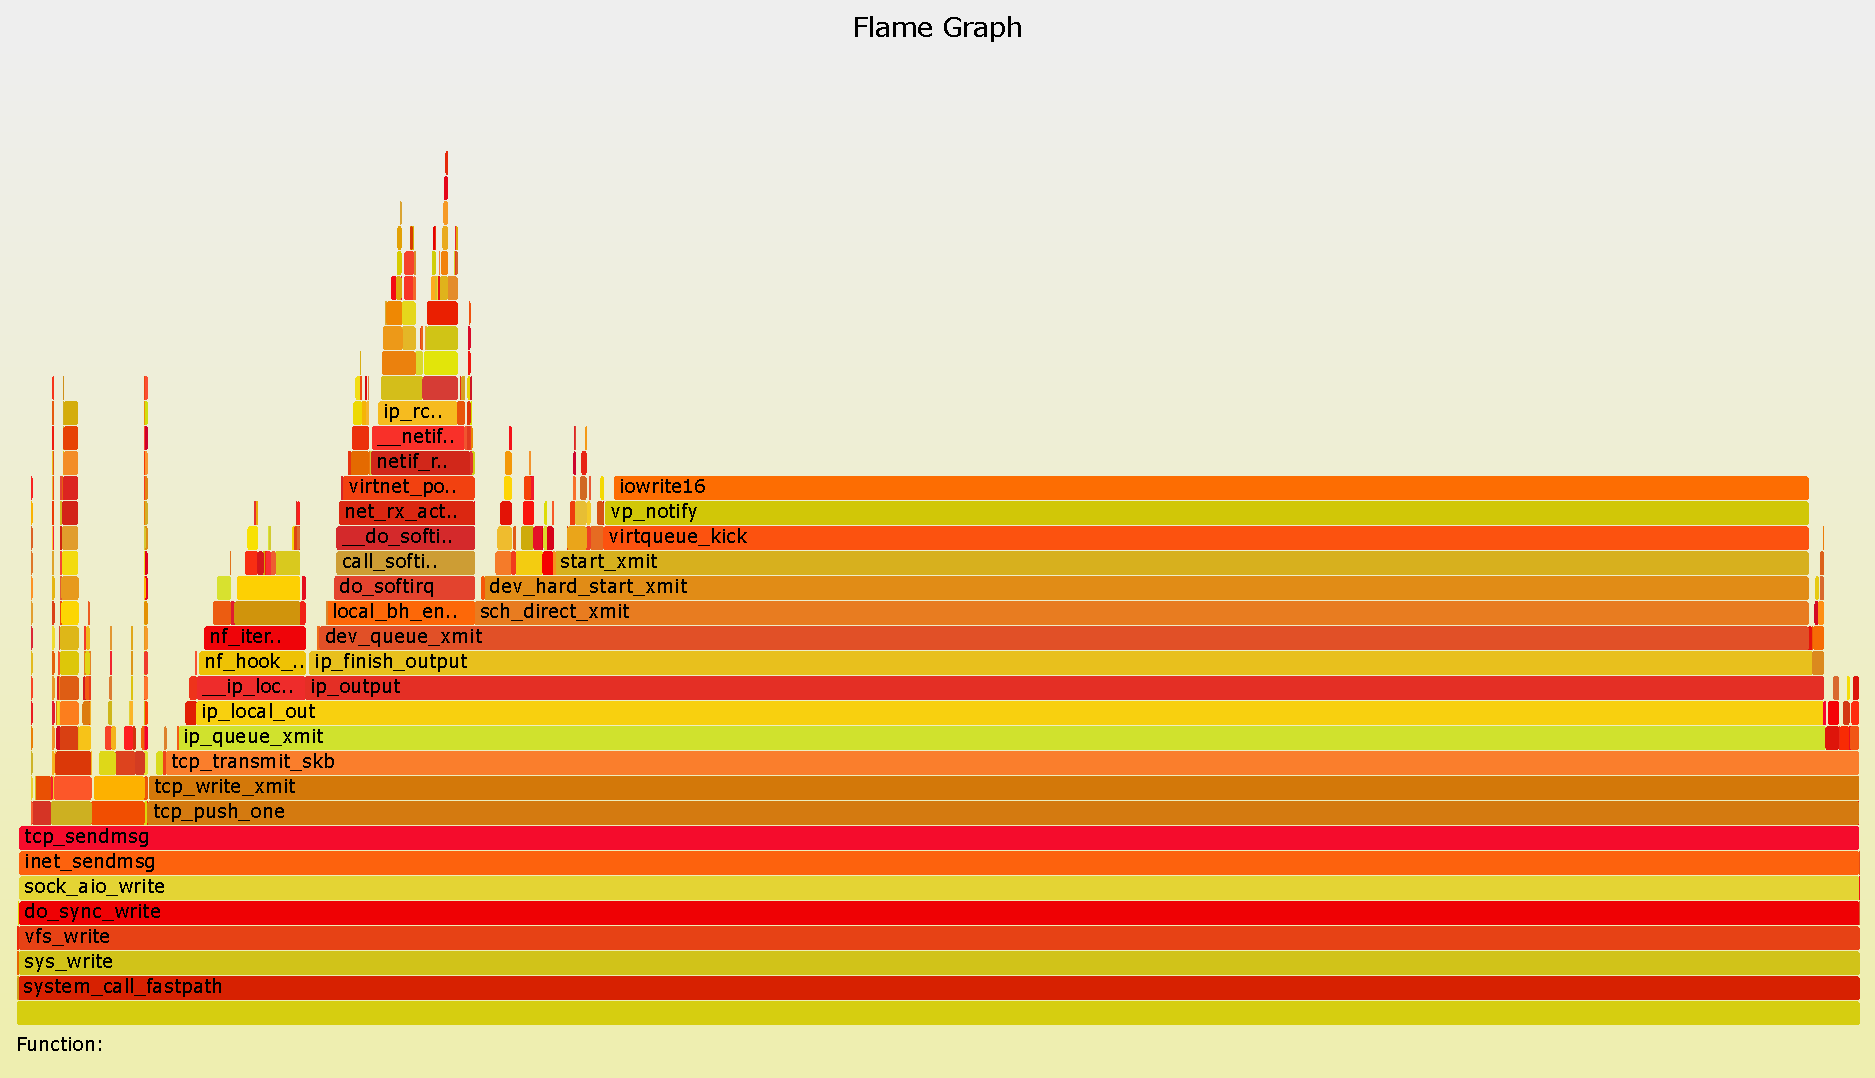
\includegraphics[keepaspectratio]{images/cpu-linux-tcpsend.pdf}}
